\label{chap:users_manual}

\section{About Filmtit Application}

\emph{Filmtit} is a web application that should assist the amateur subtitle translator with the translating the subtitles. In order to help save the amount of work spent on the translation it provides suggestions how the subtitles can be translated based database of existing already translated subtitle. Similar to Google Documents every single user operation is saved right after it is done -- there is no need for saving manually the documents, even if your browser crashes you can continue working on the subtitle document exactly at place you ended the last time.

To run the application you a web browser with HTML5 support (Opera v.12
Firefox v.14, Chrome v.21, Safari v.5.1.5 or higher \todo{find versions exactly}). If you want also use the video playback in your browser you need to have installed Java (version ???) and the VLC plugin for ??? (version ???).\todo{add it, who knows it}

\section{Registration and Login}

We require the users to be logged in to the application during their work. We do so to enable the users to save their work a return to it another time. 

\subsection{Registration and Basic Login}

First option how to get an account to the application is to register and get a user name and password. Anyway, if you have a Google or Seznam account we recommend you to use the second way of registration, via those two services.

\begin{figure}
\begin{center}
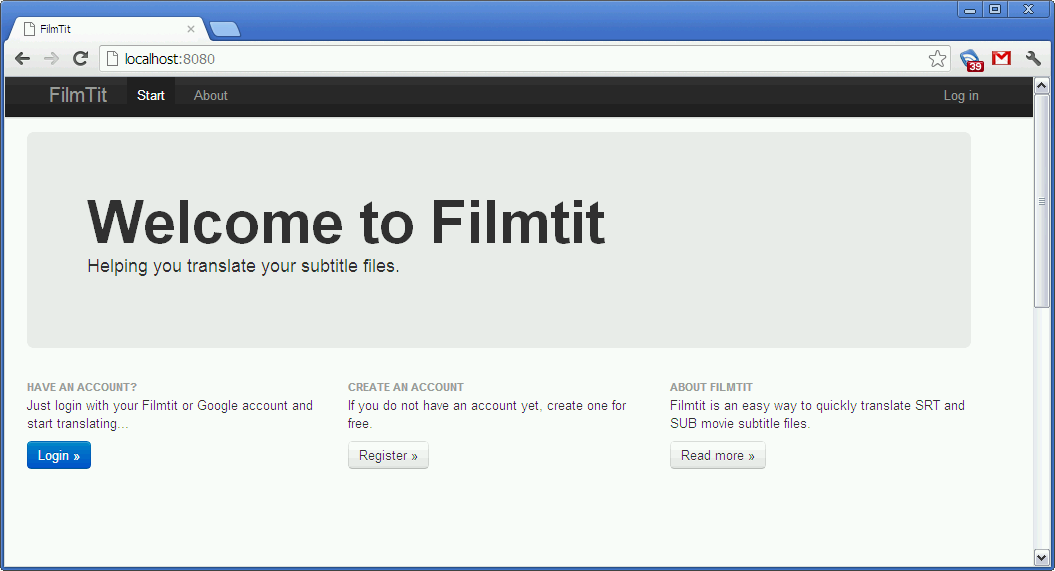
\includegraphics[scale=0.4]{figures/user_manual/welcome_screen.png}
\end{center}
\caption{Welcome screen of the application.}
\label{fig:welcome}
\end{figure}

After opening the welcome screen click on the welcome screen (figure \ref{fig:welcome}) or clicking on login button and selecting the first tab in opened dialog (figure \ref{fig:register_login}).

After that you are requested to choose a user name, fill in a valid a email address and type twice the password you would like to use. Because the application does not contain any sensitive information we try to keep the registration and login process as simple as possible and there are no requirement on the strength of the password. After the successful registration you will receive an email confirming the registration.

\begin{figure}
\begin{center}
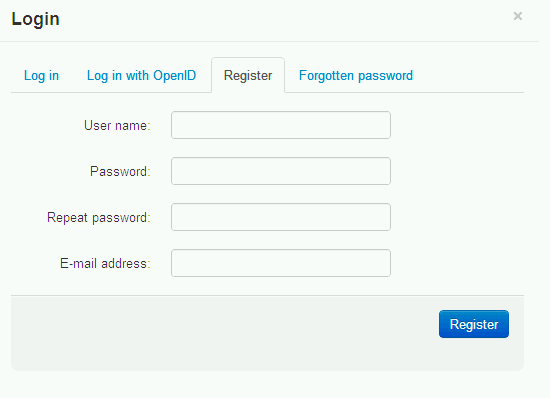
\includegraphics[scale=0.4]{figures/user_manual/register.png}~~~~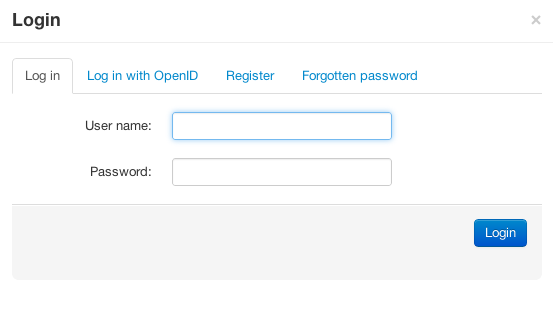
\includegraphics[scale=0.4]{figures/user_manual/login.png}
\end{center}
\caption{Registration form and login form.}
\label{fig:register_login}
\end{figure}

You are automatically logged after the registration. For logging in next time, click on the login button on the welcome screen and fill in your user name and password (figure \ref{fig:register_login}). If you want to be logged in permanently see you change it in your settings, see section \ref{sec:settings}.

\subsection{OpenID}

Another option how to log in to the application is using Google, Yahoo or Seznam account. After choosing the service you want to use a pop-up window is opened. It may happen that your browser blocks this window. If it happens you need to allow the pop-up window to continue the logging process.

You will see the login form of the service you have chosen. If you are already logged in the service you will see just the confirmation request to allow the Filmtit application to access your account data (it is your user name, first name, surname, email and gender, depending on what you filled in in the particular service and what you allowed to be provided to the third party applications, but it is never the password to the original service). After submitting your user name and user password and confirming that the Filmit application can receive your authentication data the pop-up window will be automatically closed. Within few seconds after that you will be redirected to the list of documents you own. Is is empty at the time first you log in.

You are registered automatically on first successful login. You also automatically get a user name and password for the Basic Login, which is sent to your e-mail address upon registration (if your OpenID provider provides us with one) and can be changed in the Settings.

\subsection{Forgotten Password}

Another issue connected to login is the dealing with situation when a user forgets his password. If such situation happens to you, open the login dialog and click on the "Forgotten password" tab. Fill in either your user name or email (or both) and click "Send password change link to email" (see figure \ref{forgotten_pass}).

\begin{figure}
\begin{center}
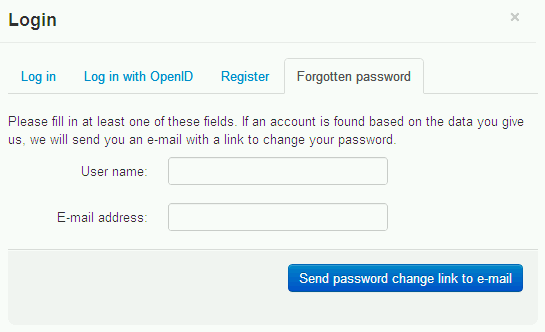
\includegraphics[scale=0.4]{figures/user_manual/forgotten_password.png}
\end{center}
\caption{Form for requesting the forgotten password.}
\label{fig:forgotten_pass}
\end{figure}

After that you will receive an email reminding your user name with a link to the page where you change your password. If you ignore the email, the old password will remain still valid.

\section{Changing the User's Settings}
\label{sec:settings}

You can change the user settings by clicking on the Settings links in the top line of the application after you are logged in. You can see the settings form in figure \ref{fig:settings}. After you are done with changing settings, click 

\begin{figure}
\begin{center}
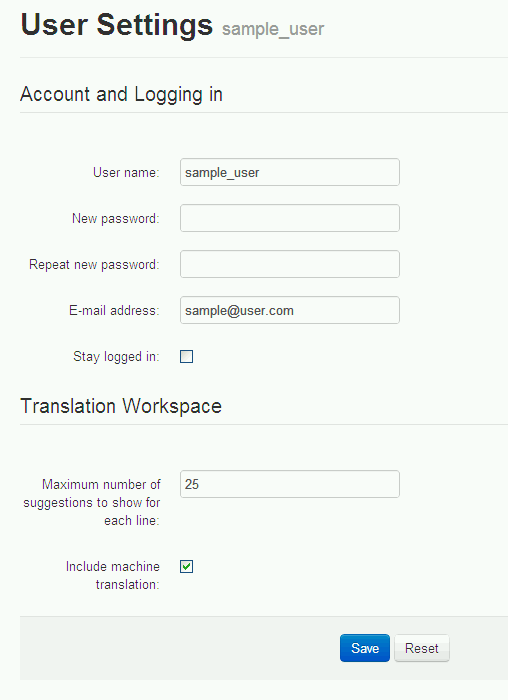
\includegraphics[scale=0.4]{figures/user_manual/user_settings.png}
\end{center}
\caption{The settings form}
\end{figure}

\subsection{Account and Logging in}
\subsubsection{User name}

You can change you user name by typing a different one. The user name has to unique within the Filmtit application, anyway if you pick up an already existing user name, the system will propose to you a similar user name which is still free.

\subsubsection{New password}

You can change your password by filling the two boxes with two identical strings which will become your new password. As was already mentioned we do not have any requirements on the strength of the password except of non-emptiness. 

By leaving the two input boxes empty, the old password remains.

\subsubsection{E-mail address}

In this input box you can change you email address. It is checked whether the address as a valid email format, but we do not test the email address availability. We recommend to fill in a working email address for the case you would forget your password.

\subsubsection{Stay logged in}

By ticking this option you be stay logged permanently logged in to the application. After a long time of not appearing in the application you will be automatically logged out (it is a month be default, but it depends on the administration settings of the server).

\subsection{Translation Workspace}

There are also some option concerning the translation workspace available. To fully understand the options, please read section \ref{sec:document_editing} first.

\subsubsection{Maximum number of suggestions to show for each line}

It is the maximum number of suggestion that can be displayed for a particular subtitle chunk being translated. It can be any number between 1 and 100. To work efficiently with the translation suggestion, we recommend to use at most 25 suggestions.

\subsubsection{Include machine translation}

By this option you indicate if you want to include automatic translation among the translation results. If this option is disabled you receive only sentences which has occurred before in subtitle files.

The machine translation are automatically generated sentences by an open-source statistical machine translation system called Moses. When we tested it on the subtitle data it performed better than the popular Google Translation (tested in August 2012). Anyway, there may situations, like movies having very specific vocabulary where it may better to switch machine translation off.

\section{Creating a New Document}

In the application we call a subtitle file as document. Creating a document means loading a subtitle file in the source language and starting translating it. You can create a new document either by clicking on the "Create a new document" button in the document list or by clicking the "New document" link in the top line.

\begin{figure}
\begin{center}
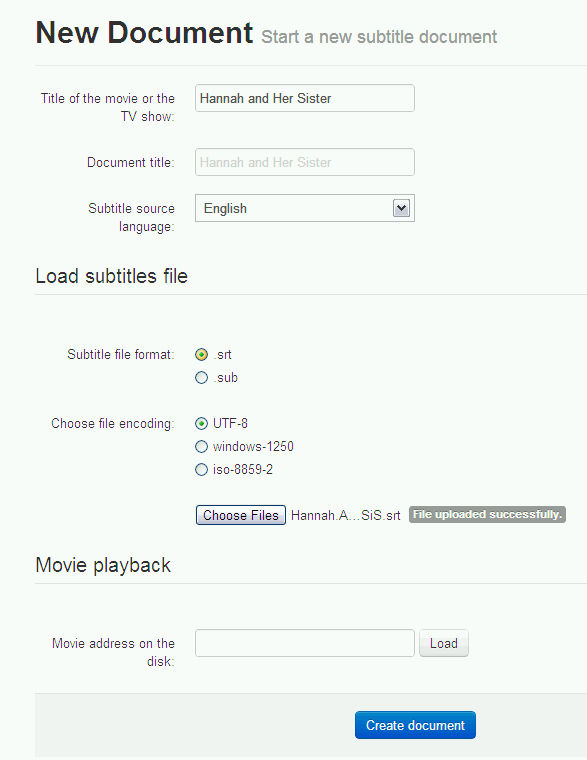
\includegraphics[scale=0.4]{figures/user_manual/new_document.png}
\end{center}
\caption{Form for creating a new document.}
\end{figure}

While creating a document you are asked to fill in the movie title and a document title in case you want to name it differently than the movie title. In the case of TV series please fill in the name of the series, not the name of the particular episode. An example of it can be to type "Lost" as the movie title and "Lost S01E01" as a document title. The you are asked to choose the source language of the subtitles, encoding of the subtitle file and the path to the actual subtitle file you would like to translate. You should also make sure you selected the proper encoding of the source subtitle file. You can choose from UTF-8, windows-1285 and iso-8859-2 which are the most commonly used encoding for Central European languages.

There is also an option to play the video of the movie you have on your computer. If you want to do so, click the "Load" button below the "Movie playback" headline and select the movie file. For this step you need to have installed Java and the VLC plugin as was mentioned before. Please be patient while doing it, loading the open file dialog can take few minutes on the slower computers. The browsers do not normally support opening the local files without posting them to the server, therefore we had to develop a non-standard solution.

Then you can submit the document creating. Within few seconds a form containing suggestion movies with title you provided should appear (see figure \ref{fig:media_sources}).

\begin{figure}
\begin{center}
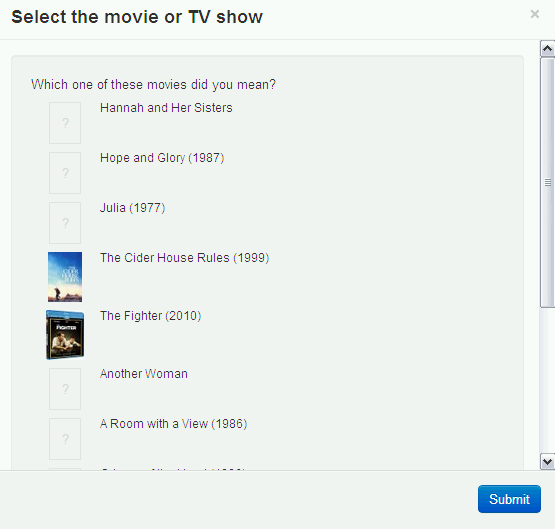
\includegraphics[scale=0.4]{figures/user_manual/media_sources.png}
\end{center}
\caption{Form for selection of a movie. It shows the suggestion after a misspelled title of Woody Alan's movie "Hannah and Her Sisters" was submitted.}
\label{fig:media_sources}
\end{figure}

After clicking on the movie you meant click submit and you can start editing your new document. In case you don't like the suggested movies at all you can click the cross in the top right corner of the form and try to reset the movie later in the document list.

\section{Document Editing}
\label{sec:document_editing}

When you start editing a document, either a new one or an existing one, you see the translation workspace, see figure \ref{fig:translation_workspace}. It has three columns. In the first column there are the timings of the subtitles, in the middle column there are the subtitles in the original language and in the third column there are the text boxes ready to be filled in by the translation in the target language.

Immediately after you open the translation workspace the translation suggestions stars to be loaded.  ...

\begin{figure}
\begin{center}
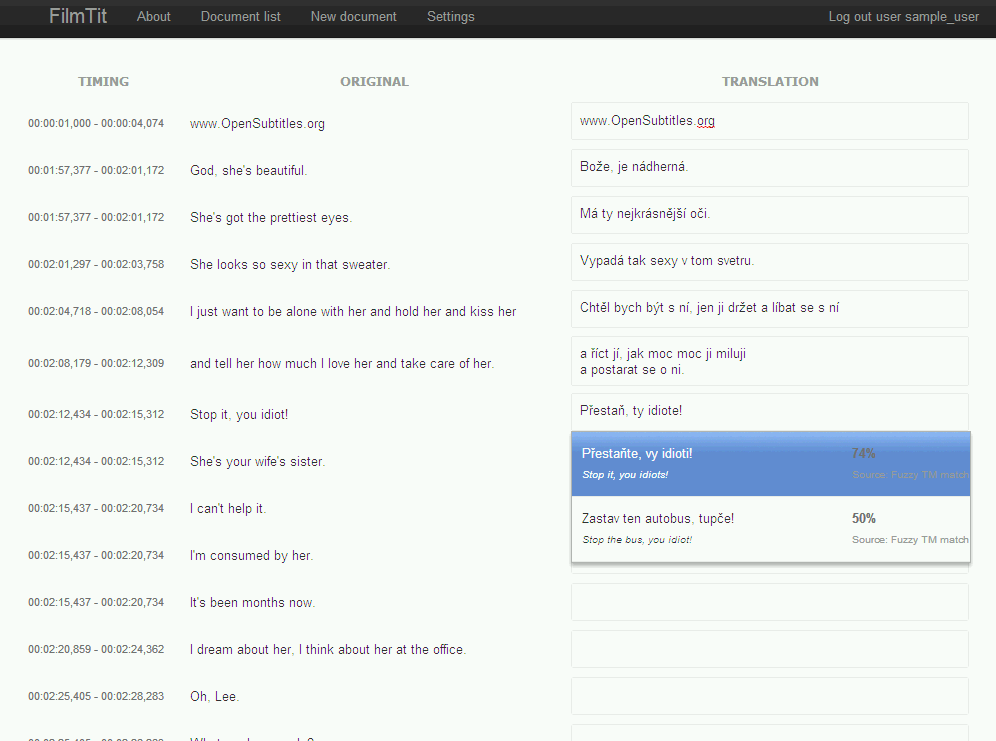
\includegraphics[scale=0.4]{figures/user_manual/translation_workspace.png}
\end{center}
\caption{The translation workspace during translating a document.}
\label{fig:translation_workspace}
\end{figure}

After the translation suggestions arrive to the translation workspace you can write down your translations.  (You can edit it even if the suggestion does not arrive, but will not be able to see the suggestions.) The translation suggestions appear below the text area where the text cursor is in. You can select one of the suggestions by clicking on them or using the arrow keys and post edit it then. You can also write the translation from scratch and ignore the suggestion. You can add a line break by pressing \emph{Enter}.

To move to the next subtitle chunk just click to the next text box a pres the \emph{Tab} key. If you want to move to the previous subtitle chunk, press \emph{Shift + Tab}.

You can change the subtitle timing double clicking on it or the text of the original subtitle also by double clicking on it. If you change the suggestion for the particular subtitle are regenerated. It may take some time to the new suggestions to appear.

It is not necessary to save your work in any way, everything is save right after it is done, so you can leave the document by clicking on a link or even close the browser and nothing will be lost. If the Internet connection breaks down you can continue working on the in the Offline Mode which is described in the following section.

\section{Offline Mode}

After the application realize it cannot to the server it offers you to continue in the Offline Mode (see figure \ref{fig:start_offline_mode}). You can continue with editing the document but you can list the documents, open another document or create a new one, neither export or delete the documents. If you refuse starting the Offline Mode, all the editing done when the Internet is down will be lost.

\begin{figure}
\begin{center}
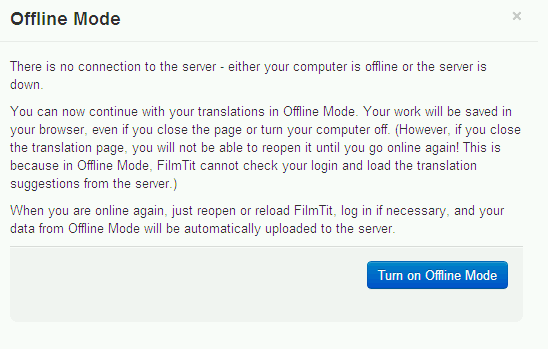
\includegraphics[scale=0.4]{figures/user_manual/offline_mode.png}
\end{center}
\caption{Confirmation request for start the offline mode.}
\label{fig:start_offline_mode}
\end{figure}

During the work in Offline Mode, all the operations are stored in the browser. Once you leave the page with the translation workspace you cannot continue editing the file, but you can even close your browser or restart the computer and all changes that you have made on the document will be saved.

The information in the Offline Mode are bound to computer, browser and user. So, to be able to upload the Offline changes to the server you have to logged in on the same computer as the same user a use the same browser.

The data from the Offline Mode are posted to the server at the time you log in to the application next time after you confirm you want to do so (see figure \ref{fig:offline_loading}). If your Internet connection starts to work during your work in Offline Mode, you can just reload the page, log in and continue with your work.

\begin{figure}
\begin{center}
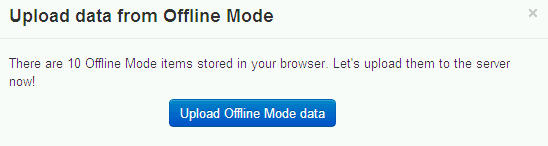
\includegraphics[scale=0.4]{figures/user_manual/upload_offline_mode.png}~~~~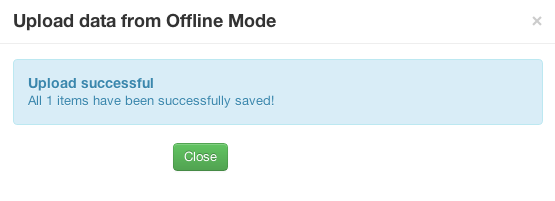
\includegraphics[scale=0.4]{figures/user_manual/upload_offline_mode_success.png}
\end{center}
\caption{Loading data from the Offline Mode}
\label{fig:offline_loading}
\end{figure}

\section{Operations with Documents}

You can list your documents by clicking on the "Document list" link in the top line of the application, see figure \ref{fig:document_list}. You can edit the document the document by clicking on the "Edit" button.

\begin{figure}
\begin{center}
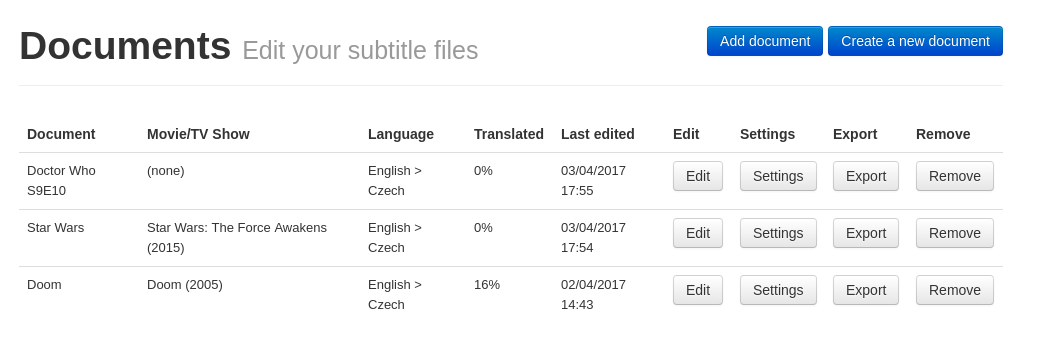
\includegraphics[scale=0.4]{figures/user_manual/list_of_documents.png}
\end{center}
\caption{List of documents owned by the user}
\label{fig:document_list}
\end{figure}

Clicking on the export button will open a dialog for downloading the subtitle file based on the document. You can select if you want to download the subtitles in the source language, the translated version or the translated version with the original subtitles where the document remained untranslated. After clicking on a button with the required format, the download of the subtitle file will start.

By clicking the delete button you will remove the document from you document list.

You can also change the title of the document, by clicking on the title and typing the original or change the movie title. If change change the name of movie, the same dialog as while creating a document will show (figure \ref{fig:media_sources}) where you can select the movie you meant.